In this section we provide an overview of PaaS clouds and Cerebro. Then we present a model for 
negotiating response time SLAs for web APIs deployed in PaaS clouds.

\vspace{-0.1in}
\subsection{ Properties of PaaS-hosted Applications}
\vspace{-0.1in}
PaaS clouds enforce a restricted programming model on the application developer to guarantee
the scalability, security and the availability of the cloud-hosted applications. 
PaaS clouds provide a predefined set of programming interfaces through which they export 
various platform services. We shall refer to these programming interfaces as the cloud software
development kit (cloud SDK). The cloud SDK exposes scalable functionality that can be used to 
program a wide range of application features. These include key-value data stores, databases, 
caching, task scheduling, and user management. In a typical PaaS environment
such as Google App Engine, AppScale~\cite{6488671}, and Microsoft Azure, 
developers use the cloud SDK to implement much of the PaaS application functionality.

Similarly, PaaS clouds may impose restrictions on performing
certain types of I/O operations, and executing long running tasks~\cite{gae-limits,azure-limits,gae-sandbox}. 
For example, Google App Engine
denies applications access to the local file system (i.e. no file I/O). Furthermore, it forces the
developer to implement all application tasks as request-response interactions of a web service
where all requests must be processed
under 60 seconds. Any task that takes longer than this is terminated by the cloud platform.
This restriction is particularly interesting to us, since it gives a 60 second default SLA
for all web APIs developed for Google App Engine.
The result of all these restrictions is a programming model that is
amenable to static analysis, a feature we exploit in the design of Cerebro. By surveying
a collection of open source PaaS applications we have also found that program features that typically
inhibit static analysis (e.g. excessive branching and loops) are rare among PaaS-hosted
applications.

\vspace{-0.1in}
\subsection{ Cerebro Architecture and Statistical Model}
\vspace{-0.1in}

\begin{figure}
\centering
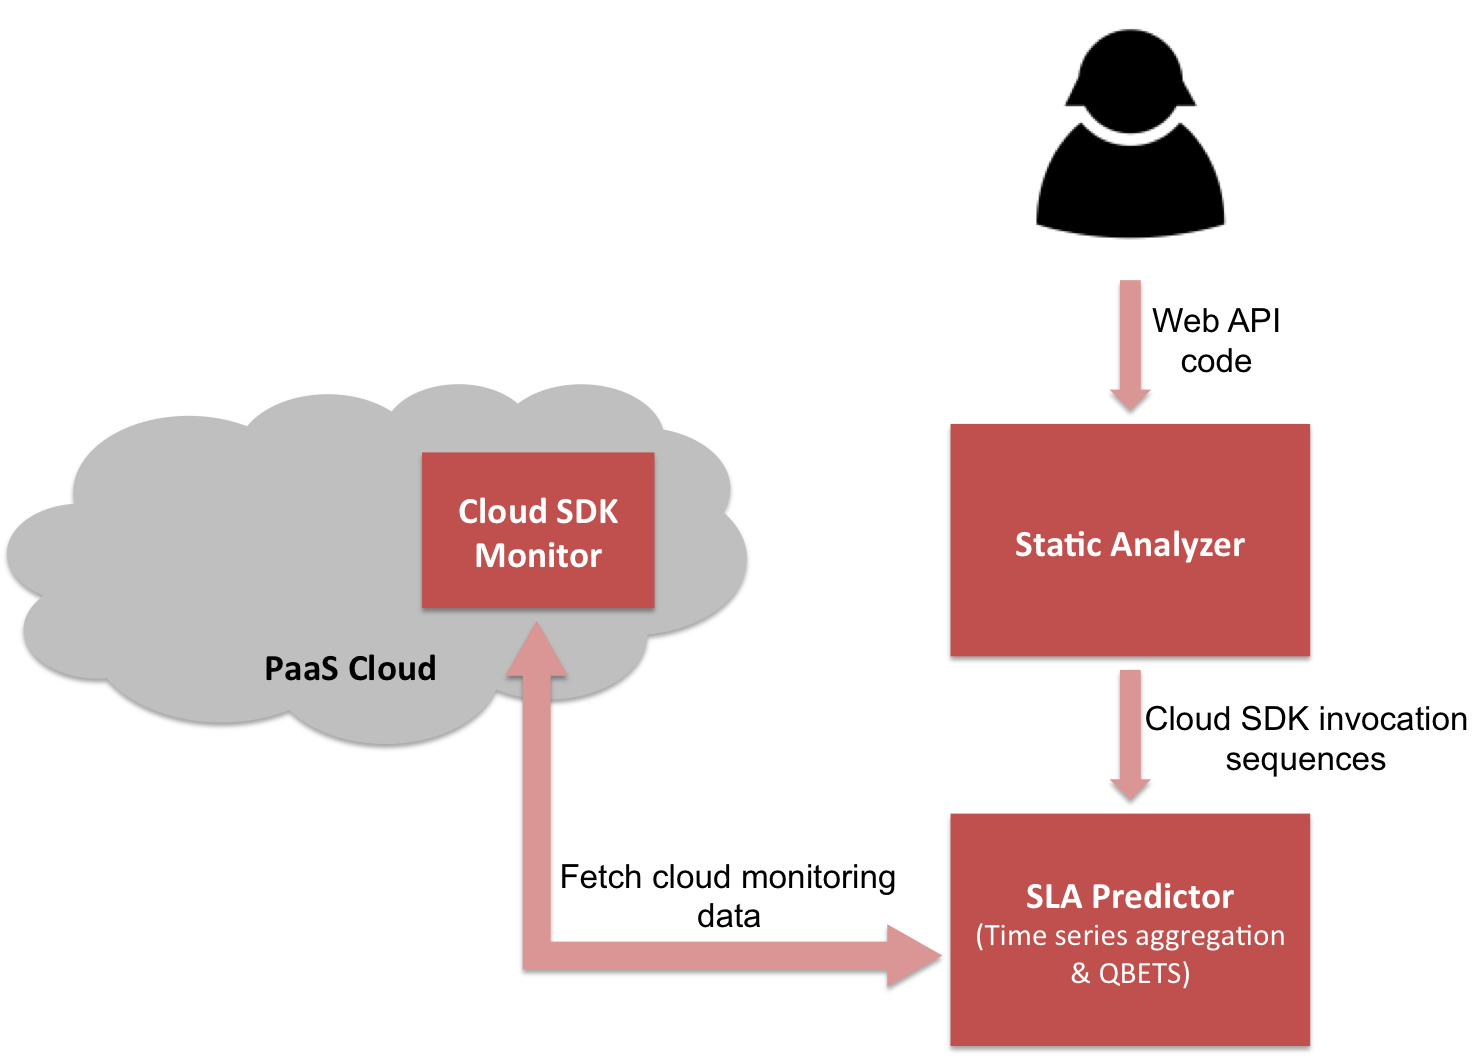
\includegraphics[scale=0.3]{cerebro_arch}
\caption{Main components of Cerebro and their interactions.}
\label{fig:cerebro_arch}
\vspace{-0.2in}
\end{figure}

Figure~\ref{fig:cerebro_arch} illustrates the main components of Cerebro, and how they interact with
each other. Cerebro runs a cloud SDK monitor in the PaaS cloud, that periodically benchmarks and records
the execution time of each cloud SDK (PaaS service) operation.
This component executes continuously and separately from all other cloud-hosted applications.

When an application developer deploys a new
application to the cloud platform, Cerebro intercepts this process and statically analyzes the 
application.  The analyzer extracts the sequence of cloud SDK operations invoked by each
web API operation in a given application. When the application code contains branches, it
extracts multiple sequences of cloud SDK operations -- one sequence per code path. The static
analyzer also looks for loops, and if any cloud SDK invocations are embedded within a loop, 
it attempts to estimate loop bounds using existing loop bound analysis methods~\cite{bygde2010static}. 
%If it fails, Cerebro prompts the application developer to provide a reasonable upper
%bound for the loop count. 
%Our survey results show that most of the time when loops are present in
%a PaaS application, they simply iterate through a dataset loaded from the cloud datastore. 
%Therefore, determining the bounds of such data-dependent loops is equivalent to establishing an 
%upper bound for the size of the underlying datastore.

%Having extracted the sequence of cloud SDK operations, Cerebro proceeds to invoke its SLA predictor.
Cerebro's SLA predictor contacts the cloud SDK monitor to retrieve the gathered benchmarking data
pertaining to the cloud SDK operations used in the application. The predictor aggregates
this data for the longest sequence (path through the operation) of cloud SDK calls and 
forms a single time series from benchmark results. 
Cerebro then processes this aggregate time series using QBETS (Queue
Bounds Estimation from Time Series)~\cite{Nurmi:2007:QQB:1791551.1791556}, a 
non-parametric time series analysis and forecasting technique. QBETS analyzes the given time 
series, and predicts an upper bound for its $p$-th percentile, where $p$ is configurable. The predicted
value $Q$ can be used to form a response time SLA of the form ``the web API operation responds 
under $Q$ milliseconds at least $p$ percent of the time''.

We primarily use Cerebro for predicting response time SLAs for web APIs
at deployment-time. However, our design also facilitates using
Cerebro as a development-time tool. That is, API developers can submit their work-in-progress
API code to Cerebro in order to gain a preliminary set of SLA predictions. Further, we can use
Cerebro as a runtime tool, where it periodically re-evaluates the response time SLAs for 
APIs already deployed in the cloud.

Periodic re-evaluation of SLAs is important because changes in the PaaS can occur
that invalidate Cerebro's response time predictions such that previously negotiated SLAs are violated.
Cerebro must detect when such changes occur so that API consumers can be notified and 
SLAs renegotiated.  SLA violations
can occur when conditions in the the PaaS change in non-random ways that impact 
the performance of PaaS services.  Such changes can result from congestion (multitenency), 
resource availability, and modifications to the implementations of the underlying PaaS services. 

To detect SLA invalidations occur, we extend Cerebro with a 
statistical model for detecting when a Cerebro-generated SLA becomes invalid. 
Suppose at time $t$ Cerebro predicts value $Q$ as the $p$-th percentile of
some API's execution time.  If $Q$ is a correct prediction,
the probability of API's next measured response time being greater than 
$Q$ is $1-(0.01p)$.  If the time series consists of independent
measurements then the probability of seeing $n$ consecutive values greater
than $Q$ (due to random chance) is $(1-0.01p)^n$. 
For example, using the $95^{th}$ percentile, the probability of seeing $3$
values in a row larger than the predicted percentile due to random chance
is $(0.05)^3 = 0.00012$.

This calculation is conservative with respect to autocorrelation. That is, if
the time series is stationary but autocorrelated, then the number of consecutive 
values above the $95^{th}$ percentile that correspond to a probability of
$0.00012$ is larger than $3$.  For example, in previous
work~\cite{Nurmi:2007:QQB:1791551.1791556}
using an artificially generated AR(1) series, 
we observed that $5$ consecutive values above the $95^{th}$ percentile
occurred with probability $0.00012$ when the first autocorrelation was $0.5$,
and $14$ when the first autocorrelation was $0.85$. QBETS uses a look-up
table of these values to determine the number of consecutive measurements above
$Q$ that constitute a ``rare event'' indicating a possible change in conditions.

Each time Cerebro makes a new prediction, it computes the current
autocorrelation and uses the QBETS rare-event look-up table to determine $C_{w}$:
the number of consecutive values that constitute a rare event.
We measure the time from when
Cerebro makes the prediction until we observe $C_{w}$ 
consecutive values above that prediction 
as being the time duration over which
the prediction is valid. 
We refer to this duration as the \textit{SLA validity duration}.  

%In our prior work, we experiment with a Cerebro prototype in the Google 
%App Engine public PaaS and the AppScale private PaaS.
%Our experiments from both settings show that when Cerebro predicts an SLA 
%%for some percentile $p$, the measured response time of the API is less
%than or equal to the predicted upper bound at least $p\%$ of the time. 

\vspace{-0.1in}
\subsection{ SLA Negotiation Model}
\vspace{-0.1in}
We extend Cerebro with an SLA negotiation process that invalidates SLAs at the end of the
SLA validity duration and re-establishes a new SLA for the API consumer.
API consumers acquire an initial SLA for a web API hosted by a Cerebro-equiped PaaS
as part of the API subscription process in which the consumer obtains her API keys.
As part of this process, Cerebro records the 
tuple $<API\ Consumer, API, Timestamp, SLA\ Value>$.

Cerebro periodically recomputes the SLA for the API over time for the PaaS. 
Cerebro is able to perform fast, online
prediction of time series percentiles via QBETS as more SDK benchmarking data becomes 
available from the Cerebro monitoring component.
When Cerebro detects consecutive invalidations of one of its predictions,
it considers the SLA to be violated and thus notifies affected API consumers to establish a 
new SLA.  Cerebro can suspend API access by affected API consumers until 
renegotiation occurs or simply record violations for later remediation.
Ideally however, it is desirable that the SLA be immediately and automatically 
renegotiated.  We refer to such on-the-fly
SLA changes as SLA renegotiations. 
Cerebro updates the $Timestamp$ and $SLA\ Value$ entries upon renegotiation 
in the appropriate data tuple for future reference.

There is also a second type of SLA renegotiation that is possible with Cerebro.
During periodic re-evaluation, Cerebro might also come across situations where the latest SLA is smaller
than some previously established SLA (i.e. a tighter SLA is available). Cerebro can notify the 
API consumer about this prospect, but wait for authorization from the API consumer before 
establishing the SLA. If the API consumer consents to the SLA change, Cerebro may update the
data tuple, and treat the SLA as established.
We next use empirical testing and simulations to explore 
the feasibility of the Cerebro SLA negotiation process and 
and evaluate how response time SLA duration and invalidation impact API consumers over time.

%We leave a more detailed discussion regarding implementing this model for our future work. That 
%discussion will address how API consumer and SLA records are maintained (data tuples), and
%how the communication between API consumer and Cerebro takes place. Also, an SLA negotiation
%model such as this is bound to have many interesting economic aspects. These include how the
%API price rates are adjusted dynamically when the SLAs change, and how the API provider is penalized
%when a previously established SLA becomes invalid. We leave that also to our future work. In this work
%we use empirical testing and simulations to explore the feasibility of the proposed SLA negotiation model,
%and how it would impact the API consumers over time.
